\documentclass{standalone}
\usepackage{freetikz}
\begin{document}
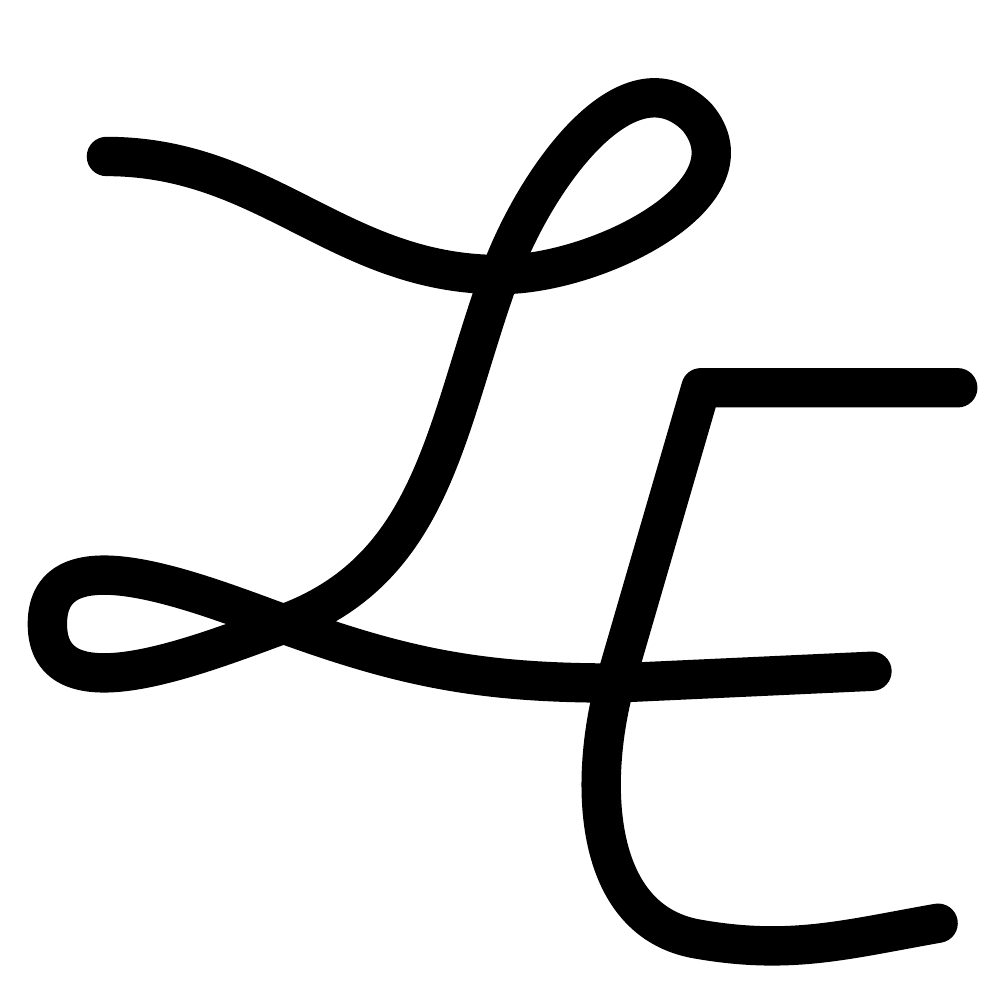
\begin{tikzpicture}
%   \draw (1, 7.5) to[out=0, in=-90] (4.5, 7.5) to[out=90, in=0] (4.5, 8) to[out=180, in=90] (3, 7.5) to[out=-90, in=0] (2, 4) to[out=180, in=-90] (1, 4) to[out=90, in=180] (1.5, 5) to[out=0, in=180] (6, 4);
%   \draw (0.5, 8) to[out=0, in=180]
%         (1, 8) to[out=0, in=180]
%         (2.5, 7.5) to[out=0, in=-90]
%         (6.5, 7.5) to[out=90, in=0]
%         (6, 8.5) to[out=180, in=90]
%         (4, 7) to[out=-90, in=90]
%         (3.5, 5) to[out=-135, in=90]
%         (3.5, 5) to[out=-90, in=0]
%         (1.5, 1.5) to[out=180, in=-90]
%         (1, 2) to[out=90, in=180]
%         (2, 3) to[out=0, in=-45]
%         (8.5, 2);
% %L 2.O
%     \draw[line width=3mm]
%         (0.5, 6.5) to[out=0, in=180]
%         % (1, 8) to[out=0, in=180]
%         % (2.5, 7.5) to[out=0, in=-90]
%         (6.25, 5) to[out=0, in=-90] %bottom of upper left loop
%             (7.5, 6) to[out=90, in=0] %far end of upper left loop
%         (6, 7) to[out=180, in=80] %top of upper left loop
%         % (4, 7) to[out=-90, in=90]
%         % (3.5, 5) to[out=-135, in=90]
%         (3.5, 3.5) to[out=-100, in=0] %TWEAK THIS TO NOT ENTIRELY VERTICAL
%         % (1.5, 1.5) to[out=180, in=-90]
%         (1.0, -0.75) to[out=180, in=-90]
%         (0, 0.5) to[out=90, in=180]
%         (1.5, 1.5) to[out=0, in=180]
%         % (2.5, 2.5) to[out=0, in=180]
%         (9, 0);
% %---------------------------------------------------------
% %L 3.O (w/E)
%     \draw[line width=3mm, line cap=round]
%         % (-0.75, 6.5) to[out=0, in=180]
%         (0.0, 6.5) to[out=0, in=180]
%         % (1, 8) to[out=0, in=180]
%         % (2.5, 7.5) to[out=0, in=-90]
%         (6.25, 5) to[out=0, in=-90] %bottom of upper left loop
%             (8, 6) to[out=90, in=0] %far end of upper left loop
%         (6, 7) to[out=180, in=80] %top of upper left loop
%         % (4, 7) to[out=-90, in=90]
%         % (3.5, 5) to[out=-135, in=90]
%         (3.5, 3.5) to[out=-100, in=0] %TWEAK THIS TO NOT ENTIRELY VERTICAL
%         % (1.5, 1.5) to[out=180, in=-90]
%         (1.0, -0.75) to[out=180, in=-90]
%         (-0.75, 0.5) to[out=90, in=180]
%         (1.5, 1.5) to[out=0, in=180]
%         % (2.5, 2.5) to[out=0, in=180]
%         (7, -0.25) to[out=0, in=185] %flatten the L to become the E middle line
%         (10, 0);
% %E
% \draw[line width=3mm, line cap=round]
%         (10.5, 3) to[out=180, in=0] %top line right
%         (7, 3) to[out=-100, in=-100] %top line left
%         %would be good to have vertical line connecting upper and middle be a straight line
%         (6.47102, 0) to[out=-100, in=180] %x=5.5 - 3*tan(10)
%         (9.5, -3) to[out=0, in=220]
%         (11, -2.5);
% % \draw (3.5, 5.5) to[out=0, in=180] (5.5, 5.5); %middle line

% %---------------------------------------------------------
% %bigger E
% \draw[line width=3mm, line cap=round]
% % (-0.75, 6.5) to[out=0, in=180]
% (0.0, 6.5) to[out=0, in=180]
% % (1, 8) to[out=0, in=180]
% % (2.5, 7.5) to[out=0, in=-90]
% (6.25, 5) to[out=0, in=-90] %bottom of upper left loop
%     (8, 6) to[out=90, in=0] %far end of upper left loop
% (6, 7) to[out=180, in=80] %top of upper left loop
% % (4, 7) to[out=-90, in=90]
% % (3.5, 5) to[out=-135, in=90]
% (3.5, 3.5) to[out=-100, in=0] %TWEAK THIS TO NOT ENTIRELY VERTICAL
% % (1.5, 1.5) to[out=180, in=-90]
% (1.0, -0.75) to[out=180, in=-90]
% (-0.75, 0.5) to[out=90, in=180]
% (1.5, 1.5) to[out=0, in=180]
% % (2.5, 2.5) to[out=0, in=180]
% (7, -0.25) to[out=0, in=185] %flatten the L to become the E middle line
% (10, 0);
% %E
% \draw[line width=3mm, line cap=round]
% (10.5, 3.5) to[out=180, in=0] %top line right
% (7, 3.5) to[out=-100, in=-100] %top line left
% %would be good to have vertical line connecting upper and middle be a straight line
% (6.47102, 0) to[out=-100, in=180] %x=5.5 - 3*tan(10)
% (9.5, -3.5) to[out=0, in=220]
% (11, -3);
%---------------------------------------------------------
%bigger E, more vertical L
%
%  _
%   \__o
%     /
%   o/_____
%
%
%
\newcommand\thicc{5mm}
\draw[line width=\thicc, line cap=round, line join=round]
% (-0.75, 6.5) to[out=0, in=180]
(0.0, 6.4375) to[out=0, in=180]
%
(5, 4.9375) to[out=0, in=-50] %bottom of upper right loop
    (7.5, 6.9375) to[out=135, in=70] %far end of upper right loop
(5, 4.9375) to[out=-110, in=20] %top of upper right loop
%
(2.25, 0.5) to[out=200, in=-90]
    (-0.75, 0.5) to[out=90, in=160] %tip of lower L loop
(2.25, 0.5) to[out=-20, in=180]
%
(6.46, -0.25) -- %flatten the L to become the E middle line
(9.7225, -0.1);
%E..................
%  Eupperleft
%     _____ Eupperright
%    /
%   /
%  (____/
%
\draw[line width=\thicc, line cap=round, line join=round]
(10.8125, 3.5) to[out=180, in=0] %top line right
(7.55, 3.5) --  %E, top line, left
% L slope = -110deg
% x=7.55 - tan(20)*(3.5- -0.25) = 6.18511
%SLOPE FORMULA DOESNT ACTUALLY WORK BECAUSE L BENDS INWARD
(6.46, -0.25) to[out=-105, in=170] %x=5.5 - 3*tan(10)
(7.5, -3.5) to[out=-10, in=190]
(10.5625, -3.3);
\end{tikzpicture}
\end{document}
